\section{Background} \label{sec-background}
In this section, we first define the required terms referring to different entities in collaborative data science platforms which we use throughout the paper.
Next, we discuss a motivating example we will use throughout the paper.

\subsection{Preliminaries and Definitions}
\textbf{ML Task.} 
To promote collaboration, the collaborative data science platforms must define the task which the users should solve.
A task specifies the requirements and the goal of the machine learning solutions.
An ML task contains the following.
(1) The type of the machine learning model, i.e., classification, regression, or clustering, (2) one or more training and test datasets, (3) an evaluation function which assigns a score to the user-provided solution.
An example of a task is to train a classification model on the training dataset $D_1$ which maximizes the F1 score on the test dataset $D_2$.

\textbf{Data and Operations.}
We support three types of data.
(1) A \textit{Dataset} which has one or more columns of data and is analogous to dataframe objects, such as Pandas dataframe \cite{mckinney-proc-scipy-2010}), (2) an \textit{Aggregate} which contains a single value or list of values, and (3) a \textit{Model} which represents a machine learning model.
The type of data is determined by the operations which generate them.
\textit{Data preprocessing and feature engineering operations}, which include simple data transformation and aggregation, feature selection, and feature extraction operations, generate either a Dataset (e.g., map, filter, or one-hot encoding operations)  or an Aggregate (e.g., reduce operation).
\textit{Model training operations} generate a Model.
A Model is used either in other feature engineering operations, e.g., PCA model for dimensionality reduction, or to perform predictions on a test dataset.
%(3) Hyperparameter tuning operations which have the task of finding the best hyperparameters for a machine learning model.
%The most common tuning approaches are grid search, random search, and Bayesian hyperparameter search \cite{bergstra2012random,snoek2012practical}.
%In all three approaches, several models with different hyperparameters are trained and the model which performs best is returned as the final result.
%In our system, instead of only returning the best performing model, we also capture all the runs with different hyperparameters.
%As a result, hyperparameter tuning operations return a set of Models.
 
\textbf{ML Workload.}
An ML workload is a script or a machine learning pipeline which performs several data preprocessing, feature engineering, and model training operations. 
The collaborative data science platforms execute a workload in either a long-running process or an interactive environment using Jupyter notebooks \cite{Kluyver:2016aa}.
%Collaborative data science platforms typically provide two modes of executions for solving tasks:
%\textit{long-running workloads} and \textit{interactive workloads}.
%The user can write an end-to-end script which performs data loading, data cleaning, and model training. We refer to this type of workloads as long-running workloads.
%Depending on the size of the initial data, a long-running workload may take anything from seconds up to many hours.
%The other type of workloads is more interactive.
%Typically, through Jupyter notebooks, collaborative data science platforms allow users to write their analysis in an interactive fashion, whereupon execution of each operation (or group of operations), they can view the result and fine-tune their analysis code.
%We refer to this type of workloads as interactive workloads.

\subsection{Motivating Example}\label{subsec-motivational-example}
Kaggle is a data science competition platform which enables organizations to host data science challenges.
Users participate in the challenges, write solutions, and submit these solutions to the platform.
To arrive at their final solutions, participants utilize the infrastructure provided by Kaggle to write data analysis and machine learning workloads either in the form of R and Python scripts (a long running workload) or Jupyter notebooks (interactive workloads) and execute them on Kaggle's platform.
Users can also make their workloads publicly available to other users.
As a result, many Kaggle users work together to find high-quality solutions.

Kaggle utilizes docker containers to provide isolated computational environments called Kaggle kernels and groups these kernels by competitions.
Figure \ref{example-use-case} shows the infrastructure of Kaggle.
Each kernel has limited CPU, GPU, disk space, and memory (i.e., 4 CPU cores, 16 GB of RAM, 5 GB of disk space, and a maximum of 9 hours of execution time. GPU kernels have 2 CPU cores and 13 GB of RAM\footnote{https://www.kaggle.com/docs/kernels}).
In busy times, this results in users to be placed in queues (especially for GPU-enabled machines) until resources become available.

\begin{figure}
\centering
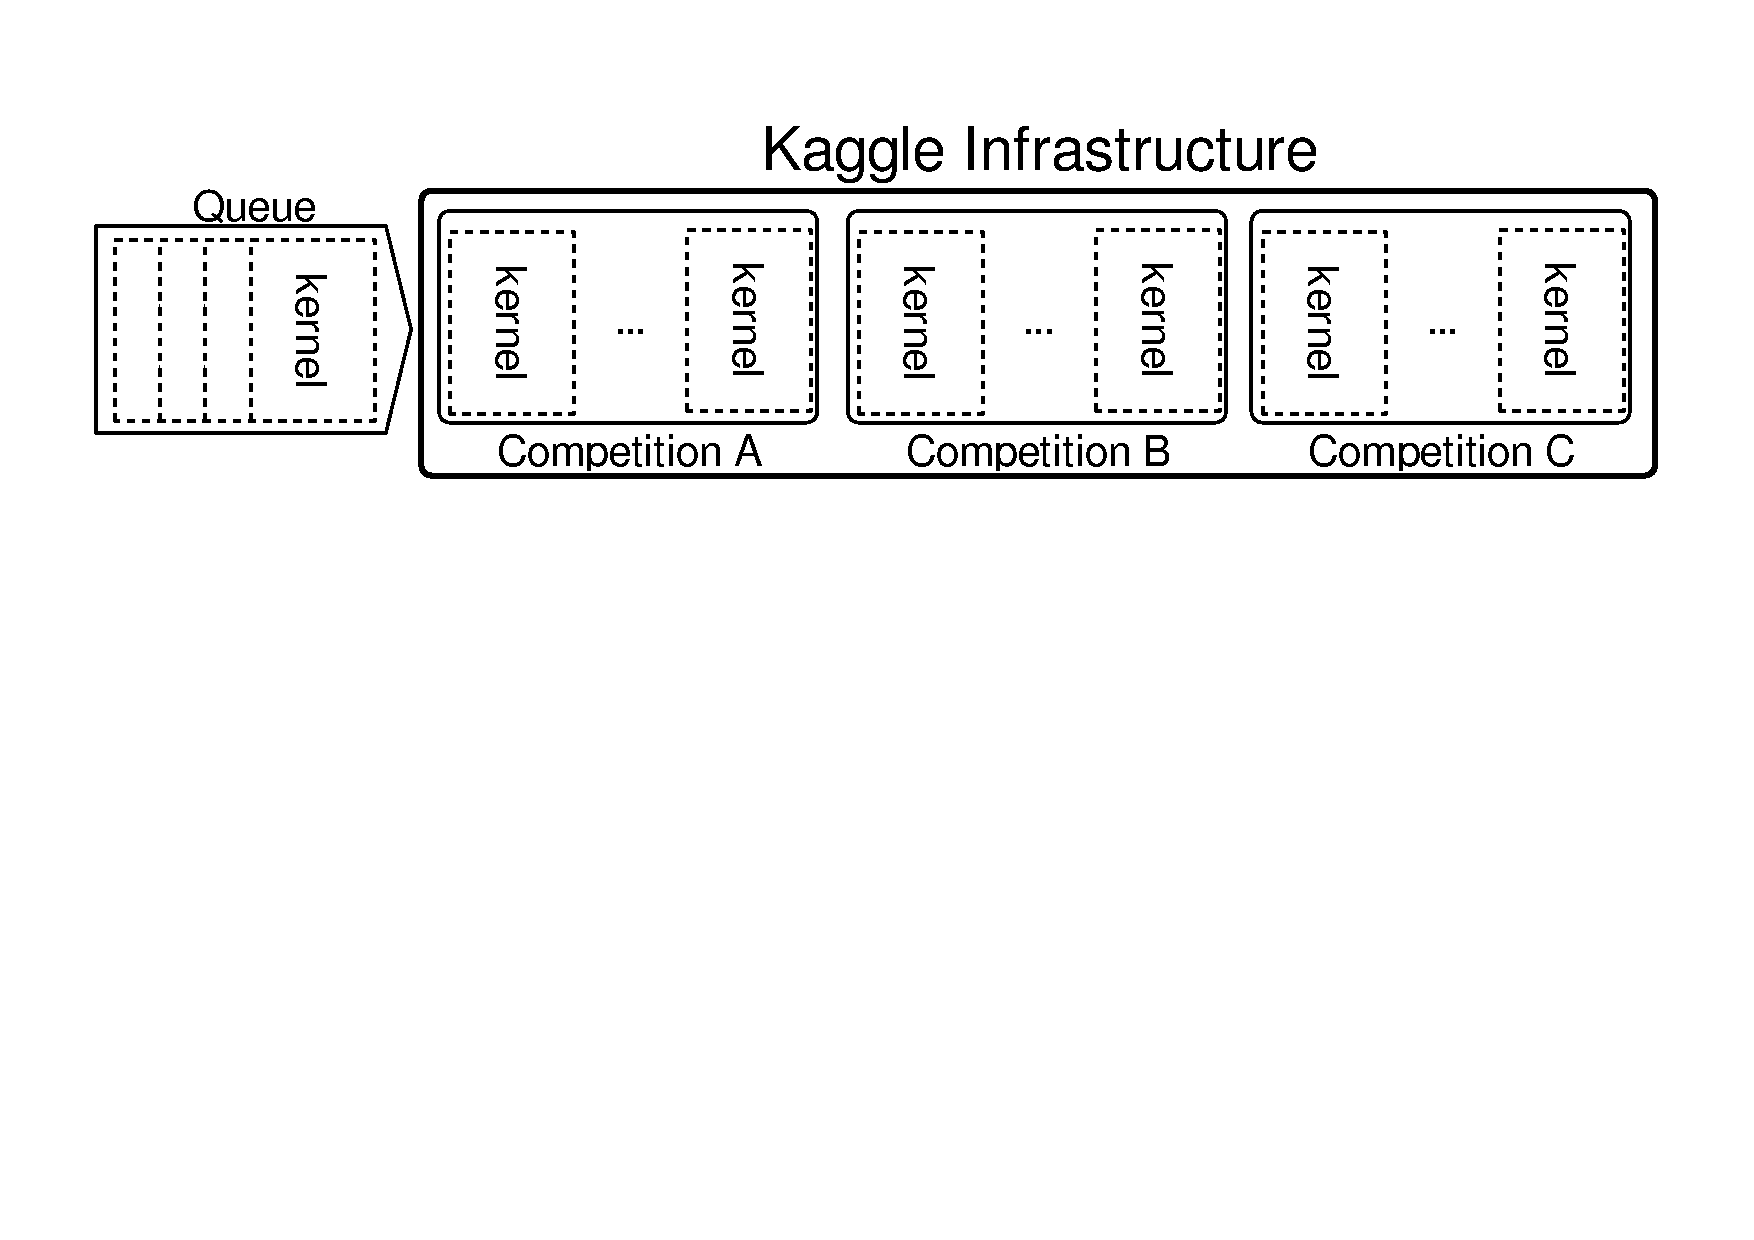
\includegraphics[width=\columnwidth]{../images/example-use-case}
\caption{Kaggle Infrastructure}
\label{example-use-case}
\end{figure}

Every user who participates in a Kaggle competition has the same goal, which is to solve the task described by the competition organizer.
Typically, the task is to design a machine learning workload containing a series of exploratory data analysis steps to preprocess one or multiple raw datasets provided by the competition organizer, followed by a model training step to train a machine learning model, which aims to maximize a quality metric on an evaluation dataset.
For example, in the \textit{Titanic: Machine Learning from Disaster} competition in Kaggle\footnote{https://www.kaggle.com/c/titanic}, the task is to create a machine learning pipeline and train a classification model on the Titanic training dataset that can predict if a traveler survived the Titanic disaster, with the goal of maximizing the prediction accuracy on a separate test dataset.
When solving the same tasks, users tend to utilize the same type of operations.
Figure \ref{fig-titanic-script-hierarchy} shows the most popular kernels and their relationship for the Titanic competition.
% Tilmann: seems that this is something you define? how does this help your analysis? Behrouz: I'm trying to motivate the fact that people implicitly or explicitly use similar operations. Here, 'relationship' mean when an author explicitly cites another work in his script.
\begin{figure}
\centering
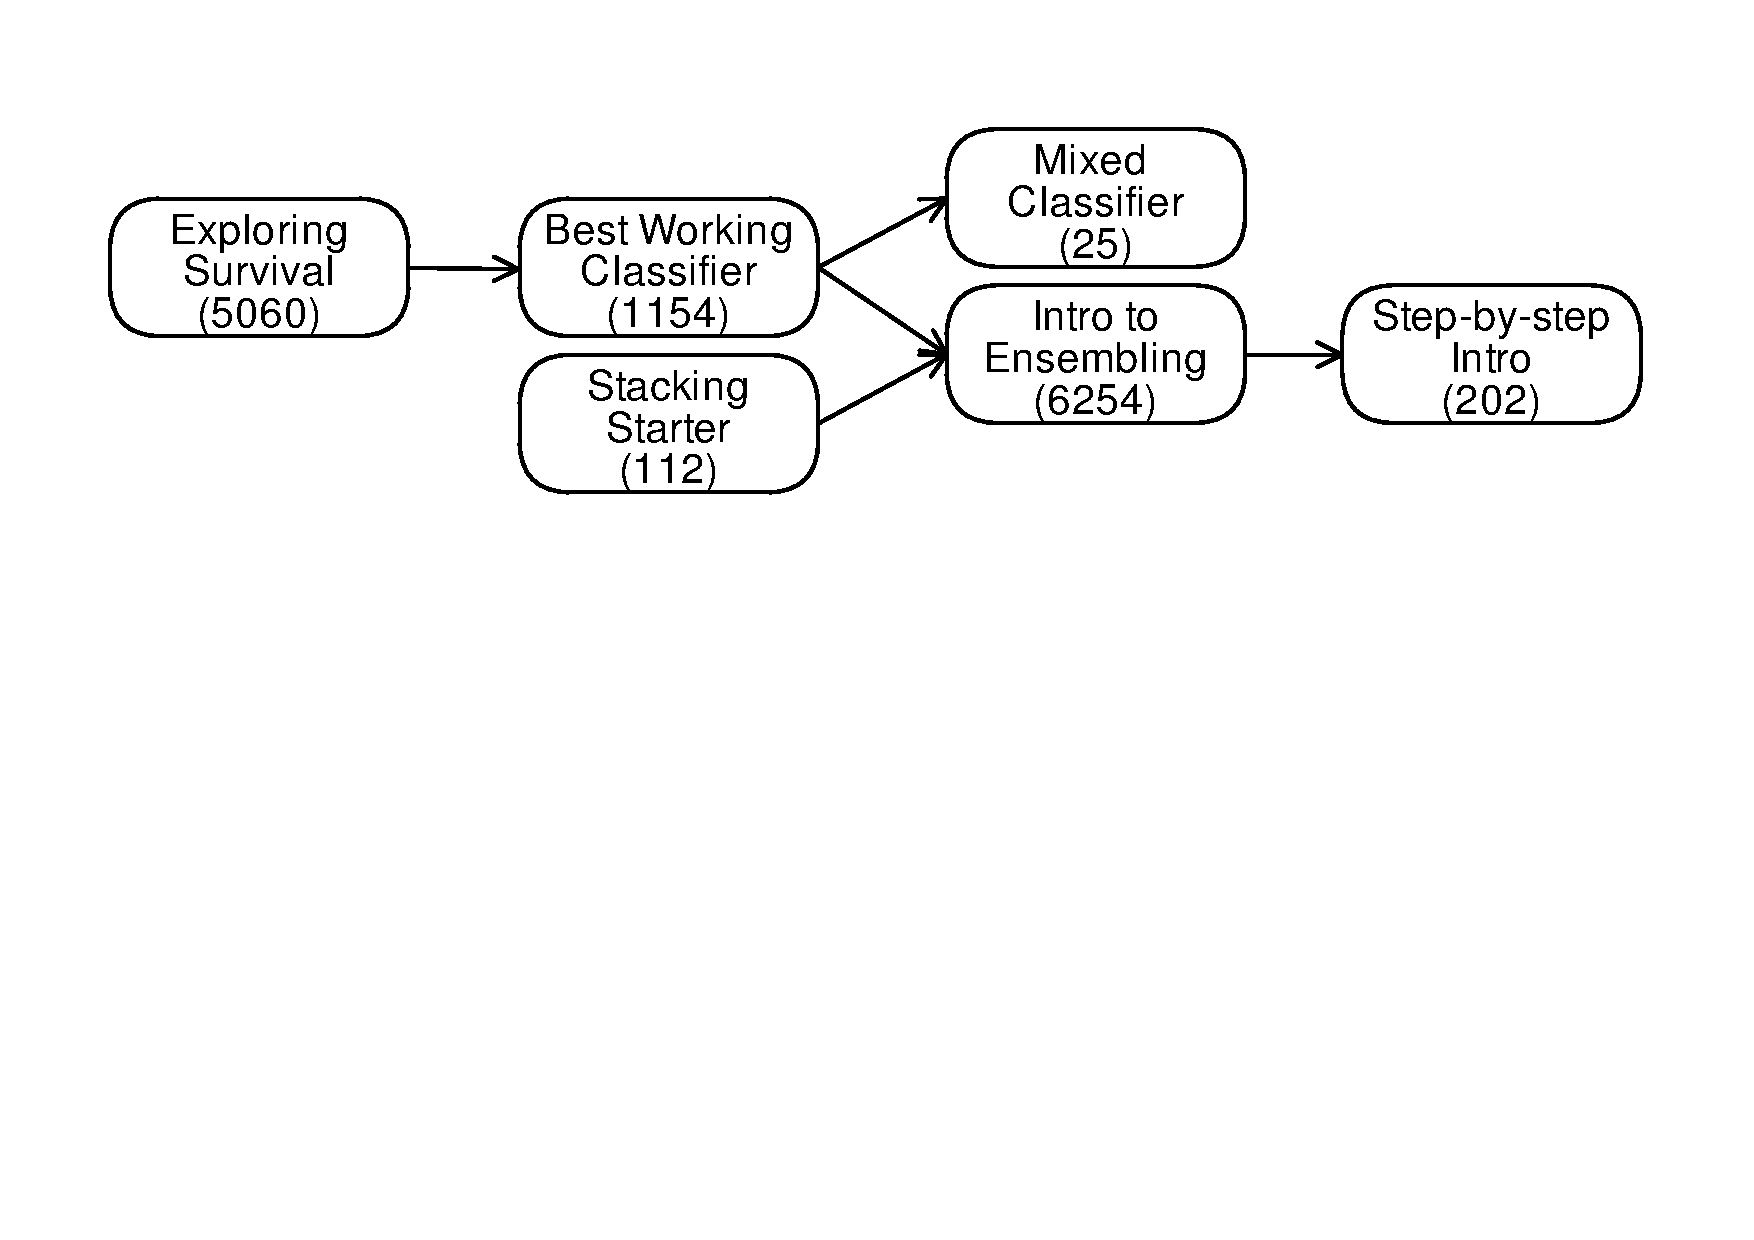
\includegraphics[width=\columnwidth]{../images/kaggle-titanic-scripts-graph}
\caption{The fork hierarchy of some of the popular kernels in Kaggle's Titanic competition}
\label{fig-titanic-script-hierarchy}
\end{figure}
For example, in the kernel \textbf{Best Working Classifier}, the author explicitly cites the kernel \textbf{Exploring Survival} as his/her inspiration.
The numbers show how many times other users copy a kernel into their workspace.
%TODO this number is pretty old, I should update it (or better yet do one figure from the competition that I'm using for the experiment (i.e., home credit)
The most popular kernels for the Titanic competition have been copied a total of 44,434 times.
This demonstrates that many of the executed workloads share exact or similar operations.
Since Kaggle is using isolated docker containers for executing user workloads, they cannot detect similar operations and re-execute the operations multiple times.
Moreover, while users can view and study publicly available kernels, they are not able to directly access the intermediate artifacts, such as any preprocessed dataset or machine learning model belonging to the existing kernels.
As a result, users must re-execute a kernel to generate the desired artifact.


%\subsection{Experiment Database}
%Experiment databases include data and meta-data of different data analytics and machine learning experiments executed over time \cite{miao2018provdb, vanschoren2014openml, schelter2017automatically, vartak2016m}.
%They include different information about datasets, data processing pipeline components, machine learning models, execution of machine learning training algorithms, and quality of the models. 
%Moreover, some experiment databases allow users to store some of the artifacts generated during the execution of a workload, such as raw datasets, intermediate datasets (resulting from applying data transformation operations), and machine learning models and their hyperparameters.
%However, due to limited storage space, experiment databases cannot store every artifact.
% 
%Experiment databases can help in designing a better future workload.
%For example, users can query the database to find the answer to the following questions: what type of data transformations and model training operations are executed on a dataset and what is the accuracy of the final models?
%As a result, users can avoid executing data transformations or model training operations that do not result in high-quality models.
%Moreover, experiment databases enable reproducibility and validation of results.
%For example, users can query information about the environment and list of operations in a specific workload.
%As a result, users can re-execute the workload and compare the results.